\chapter{An Approach for Reproducible Analysis}

\begin{center}
  \textit{If you're doing an experiment, you should report everything that 
    you think might make it invalid - not only what you think is right about it; 
    other causes that could possibly explain your results; and things you 
    thought of that you've eliminated by some other experiment, and how they 
    worked - to make sure the other fellow can tell they have been eliminated.}

 - Richard Feynman
\end{center}



A strategy is needed to facilitate reproducibility of NMR data analysis.
This chapter will describe in more detail the common characteristics of
the missing data and what role they play as well as why it is important to
capture them, a model for capturing that data, and a strategy for using
the model during the analysis process.


\section{Missing data and its role in analysis}

% need to cover what the data is, how it plays a role in NMR analysis, 
% why it's important to capture
As was described in earlier sections, 
spectral analysis, including peak picking, GSS construction, GSS and resonance
typing, sequential GSS assignment, and sequence-specific GSS assignment is 
accomplished using a step-by-step process of deductive reasoning 
which is often augmented by computational tools.  The computational 
results may be subject to manual validation, correction, and extension
\cite{guerry2011automated}.  This section will explore the various types
of data involved.

\subsection{Intermediate results}
An important feature of the analysis process is that the final results are
not the output of a single replicable step, but rather of a series of steps
of refinement and modification.  Thus, the analysis process implicitly 
generates a new data set (from the previous one) after every modification, 
whether manual or automated.

Implicit in the sequence of data sets are logical dependencies of derived
data upon features of the previous data set: the context of each deduction
is important, because the exact context determines what deductions may be
made and the confidence level of each deduction. % TODO an example

The importance of capturing intermediates is due to the dependence of 
deductions on context: without knowing the context, it is impossible to 
evaluate the correctness, confidence, and alternative interpretations of
a deduction.  In standard approaches to analysis, the contexts are not
captured; they are implicit.  By making the contexts explicit, it becomes
possible not only to fully recapitulate the process of analysis, but also 
to employ error detection and correction strategies by analysis
of deductions and their contexts.  
An interesting side-effect of capturing
contexts is that analysis can be restarted in the middle, by selecting an
appropriate context and applying a different deduction.

% TODO
% come up with a simple example that demonstrates: 
%   1) the dependence of deductive ability on context
%   2) the concept and utility of multiple snapshots
%   3) the concept and utility of tracking logical dependencies

\subsection{Deductive reasoning}
As was covered earlier, the deductive process of reasoning which plays
a major role in data analysis generates intermediate data sets.  Associated
with the generation of these data sets is a rule employed for deduction.

% TODO do I need to say something about the proposed library of deductive reasons? or does that come later?
Each rule is an embodiment of NMR-specific knowledge of how to interpret a
data feature.  In general, a deductive rule requires an input, produces an
output, and has an intuitive justification for its action.  
% TODO example

Application of these rules provides a rationale for manual modifications.  The
rationale is a justification that the change modification is correct, as
well as an indication of why the change was made.  Therefore, capturing the
deductive rules employed enables verification of the veracity of modifications. 
It also facilitates knowledge transfer, both in the contexts of collaboration
and teaching, by providing a meaningful annotation (with reference to the
domain of NMR) for actions taken.

\subsection{Extraneous Results}
During analysis, some portion of the positive results are not of direct interest
to the final answer.  Not only peaks, but also resonances and GSSs are included.
The positive results include both false positives, caused by noise or
artifacts, and true positives, caused by contaminants.

Although not of direct interest, such extraneous results play a role in 
the process of analysis: as was covered earlier, when making a manual
modification, a deductive rule is applied to a context (data set).  Changing 
the context affects which rules apply and what deductions are made; 
therefore, as a part of the context, extraneous results matter during analysis. 
If incorrectly identified or left unrecognized, extraneous features can
lead to incorrect peak picking, chemical shift assignments, GSSs, and GSS
assignments.

A further benefit of capturing extraneous results is the ability to distinguish
between identifying a data feature and interpreting it.  In other words, peaks
picked during peak picking are treated as positives, this is the "identification"
phase; in the later "interpretation" phase, these peaks are separated into
false positives and true positives.  This allows rectification of the 
discrepancies between uncorrected computational results and the final,
deposited results as well as marking potentially suspicious results for 
future perusal.  It should also be noted that picking a peak, then
interpreting it as extraneous and discarding it is typically not reported in
final data sets, despite containing important information.
There is a balance between false positives and false negatives \cite{pine};
false negatives are more undesirable \cite{pine, saga, guntert2009automated},
and capturing extraneous results helps to avoid this tradeoff: by reducing
the cost of a false positive, tools are free to focus on avoiding false
negatives.

The process of separating positives into false and true is prone to 
introducing bias; by keeping and reporting the initial results, such bias
can be estimated.  This is not possible if the extraneous results are not
reported, and also allows the feature identification phase to proceed
without bias, since error correction will be applied at a later stage. 
By providing additional context, it may be possible to estimate the quality 
of an analysis, where errors may be most likely found in the borderline 
cases; it will also help assigning confidence levels to datums by not.
Additional quality measures enabled include the number of peaks found by the
peak-picker, the number of false positives, the number of peaks assigned to
GSSs, and the number of GSSs assigned to residues.  It may also be possible
to estimate contamination, incompleteness and overcompleteness, overfitting, 
and consistency.

\subsection{Notes}
Due to the difficulties inherent in data analysis, situations are reached
in which the interpretation of a specific feature is problematic:
\begin{itemize}
  \item uncertain or impossible.  The evidence for a particular deduction 
    is not solid.
  \item ambiguous.  Multiple interpretations of a feature are consistent
    with the data and satisfy the constraints.  It is not possible to choose
    between them.
  \item inconsistent.  The data set is in an inconsistent state, or a 
    deduction would leave it in an inconsistent state.
\end{itemize}
A simple example is non-stereospecific sidechain proton assignments: 
a residue such as a Histidine or Lysine which has two beta protons will 
often give rise to two resonances, one for each beta proton; however, 
without additional information, it is impossible to assign a resonance to
a specific atom.  A related example is caused by the two delta and epsilon
protons in Phenylalanine and Tyrosine aromatic sidechains; the two resonances,
even if distinguishable, can not be uniquely assigned to atoms.  In both
cases, the ambiguity is resolvable through the use of additional information;
however, before that additional information is provided, it is useful to be
able to store what is known -- that there are two peaks, each of which 
corresonds to one atom, but exactly which is unsure -- as an indication to
future analysis or perusal that a problem has been identified but not yet
solved.

The key idea is, given the inevitability of such problems during data
analysis, to create facilities for explicitly recognizing, discussing, 
and handling such problems \cite{robillard2007concerns}. 
Several strategies for such an approach 
are covered in \cite{nuseibeh2000inconsistency} including deferral of the
problem while flagging it for later follow-up.

Enabling the representation of such data has similarities to the probabilistic
approach applied by PINE \cite{pine} to great effect.  
PINE deals with the innate uncertainty of data 
analysis by resolving the tradeoff between false positives and false 
negatives through association of a probabilistic confidence metric with each
feature interpretation; low confidence values are used as evidence that an
interpretation is suspicious and needs additional verification or data.
In a complementary approach, capturing notes of analysis issues also 
resolves the tradeoff for manual analysis, by enabling the association of
an explanatory or warning message with suspected low-quality deductions.
In addition, the message may contain more information than a scalar: it may
necessarily refer to multiple conflicting pieces of the data set in the case
of a contradiction.

% TODO add a picture
Correctly identifying and characterizing peaks in the presence of significant
amounts of overlap is a notoriously difficult problem \cite{guerry2011automated}.
The number, position, and intensity of peaks become distorted by the overlap.
In such a case, it may not initially be possible to fully and correctly
resolve the overlap (although later information from additional spectra, such
as a higher-dimensional spectrum in which the additional dimension removes
the overlap, may resolve the problem); a note explaining that overlap is
suspected and that the characterizations may be in error points this out.

% TODO add a picture
Building unambiguous and complete sequential GSS assignments is complicated 
when multiple GSSs have the same or nearly the same chemical shift values
for resonances which are or potentially may be assigned to CA, CB, CO, or the
corresponding (i-1) atoms.  Leaving a note in the data set describing what
the ambiguity is ensures that this information is not lost, and is clearly
marked for re-analysis when more data becomes available.


\section{A Model for Reproducible NMR}

\subsection{Data models}
A data model is a means of specifying the structure of information  
\cite{codd1970relational}.  This
information may be used as inputs and outputs for computational tools, or
it may be archived and available for reference use.  Data models are useful
because they provide a formal specification of the structure, which enables
unambiguous, correct, and automated use of data.  Data models are
abstract specifications; they must be implemented in source code in order
to become a usable artifact.

In the field of NMR, both the BMRB \cite{bmrb} and CCPN \cite{ccpn} have
created descriptive, extensive and useful data models, and have implemented them 
in programs and as Application Programming Interfaces (APIs).  These are used
by additional programs to help manage the exchange of data with external
programs.

This section will cover a data model for reproducibility.  Once a data
model exists, it can be implemented as part of a software program that
facilitates reproducible data analysis, as will be covered in a later 
chapter.  The core of this data model is formed by the BMRB \cite{bmrb}
and CCPN \cite{ccpn} data models.  These models are then extended with
several additional data types and properties in order to enable 
reproducibility.

\subsection{Intermediate results}
The strategy for modelling intermediate results is based on the data models
of existing version control systems, including Git \cite{loeliger2012git},
SVN \cite{svn}, and CVS \cite{cvs}.  Figure-\ref{intermediates} shows the
general properties of the solution: a sequence of snapshots of the data set,
where associated with each snapshot is a small amount of metadata:
\begin{itemize}
 \item timestamp
 \item author
 \item parent, or previous snapshot.  This maintains the order of the 
  snapshots
\end{itemize}

When multiple snapshots are captured, they can be compared as in Figure-\ref{diff},
and also can be used to track logical dependencies of analysis.

Figure-\ref{snapshot_model} shows an entity-relationship (ER) model built
using MySQLWorkbench.

\subsection{Deductive reasoning}
A model for the deductive process of rule application to a data set to 
produce a modified, new data set requires components for both the rules 
themselves as well as the use of rules.  

A library of rules was built which enumerates deductive rules based on 
established practices during data analysis \cite{guerry2011automated, hncacb,
hnco, cbcaconh, hbhaconh, picky, xeasy, sparky, ccpn}.  For each rule, 
a meaningful name, an explanation of the rule's meaning, its intended use,
its intended result, and examples was collected.

During analysis, one or more rules are applied to make a deduction.  This
is capture in Figure-\ref{deduction_model}.

% TODO clean up library so that it's usable
% TODO present most or all of the library, in picture and textual format

\subsection{Extraneous results}
To model extraneous results, the BMRB and CCPN models \cite{bmrb, ccpn}
were extended to support additional fields which distinguished between 
extraneous and primary data.  Other than these additional pieces of data,
the models do not differ.  This applies to peaks, resonances, and GSSs.
The general approach for using this model is to never directly delete
a peak, resonance, or GSS, but rather to mark it as extraneous by modifying
its associated category from 'signal' to 'artifact', 'noise', 'contaminant'
etc.

For example, while using an interactive spectral analysis such as Sparky or
CCPN Analysis \cite{sparky, ccpn} for peak picking a spectrum, it is common
to run the automated, built-in peak picker and then to manually correct the
results by deleting some peaks and adding new ones.  This approach would
work differently; peaks would not be deleted.  If the category of each of the
peaks initially picked by the automated tool were 'signal', then the task of
the user would be to correct all of the categories for peaks which were 
determined to be signal or noise; note that these peaks would not be deleted
from the list.  They would remain in the list but with a different category
tag that would differentiate them from signal peaks.

% TODO a pictoral representation of this model
% TODO examples
% TODO 
% CCPN peak pick as initial peak list, then corrections I made as peak list 
% where each peak has additional fields

\subsection{Notes}
To model notes, the BMRB and CCPN models \cite{bmrb, ccpn} were extended
to support an additional data type: a note.  A note can refer to one or more
other feature of the data set, and also includes a textual description of
the nature of the problem, as well as an indication of how the problem might
be resolved (although that is optional).

% TODO a pictoral representation of this model
% TODO example: odd feature in data, unable to resolve


\section{An implementation of the model}
% TODO a Sparky extension


\section{Applying reproducible analysis: using the model}
This section presents some general advice for how to use the reproducibility
model effectively in practice.  It provides tips and suggestions, as well
as covering common problems and how they can be avoided.

\begin{itemize}
  \item one snapshot, one focus.  Keeping each snapshot focused on dealing
    with a single issue helps the process of analysis to remain understandable
    to later perusers.  This is because it makes the logical dependencies 
    more obvious; when a single snapshot contains many unrelated things, or
    is extensive enough that part of the snapshot depends on other parts, then
    it is no longer clear what the logical relationships are.  Keeping snapshots
    small and focused alleviates this issue.
  \item level of detail.  It is not necessary to exhaustively annotate every
    last single change; clearly, such an approach would be problematic because
    it would require far too much time and effort on the part of its users.
    Rather, the value of this reproducible approach is to clearly indicate 
    major issues and modifications.  The more important and the more time and
    brain power went into making a deduction, the more annotation it typically
    deserves -- in other words, a complicated deduction requires a complicated
    justification.  On the other hand, if multiple peaks are quickly and
    straightforwardly identified as artifactual with a minimum of effort, 
    only a bare minimum of annotation is needed; the deduction does not become
    clearer with additional annotation.
  \item apply the correct rule(s).
  \item record uncertainty and resolution.  When in doubt or difficulty 
    during analysis, record all information pertaining to the issues, whether
    as a note or extraneous data.  Even if the problem is easily or quickly
    solved, describing it creates a record of that problem which is valuable
    for later perusal.  Trends over such a record help to indicate more 
    large-scale problems, as well as illuminating troublesome spots for
    collaborators and learners.
\end{itemize}
   
% maybe talk about the culture of the lab notebook?
% could this belong in its own chapter?
% or in the software chapter, or in the 'reproducible data sets' chapter?


\section{Archiving reproducible data sets}
A major portion of the value derived from collecting reproducible data sets
is disseminating them so that others may obtain and use or inspect the data
in some way.  The standard means for sharing NMR-derived data is the BMRB
\cite{bmrb}, which uses the NMR-Star file format.  In order to enable archival
of reproducible data sets, we have collaborated with the BMRB to extend the
NMR-Star data dictionary, so that reproducible data sets may be collected and
deposited in the NMR-Star format.

The NMR-Star data dictionary, which may be found at 
\url{http://www.bmrb.wisc.edu/dictionary/}, catalogs the names, structure,
intended use, and definitions of the data types handled by the BMRB.


\section{Discussion}
By collecting reproducible data sets, the true information content used in
NMR spectroscopy is made explicit and visible.  This is analogous to how lab
notebooks are intended to be used in wet-lab work: as a means of recording
the crucial details describing how an experiment was done, so that the procedure
can be shared with and improved upon by others.  A key difference, however, is
that while lab notebooks have been in use for several centuries, the culture
of reproducibility of digital analysis is still in its infancy: we do not yet
have much experience with the what, how, and why of reproducibility in 
electronic media.

% TODO this is a pretty weak paragraph
The first key step, which I have described in this chapter, is to define what
the problems are -- in the form lost data -- and a model for what that data is.
Then the model must be applied in practice, and its correct use taught.

By extending standard existing models, the barrier to entry is greatly reduced,
and instead of requiring an abrupt and drastic change in the workflows of those
already using the standard models \cite{bmrb, ccpn}, the change to reproducible
analysis can be incremental and gradual.  This should help adoption.

Not only will such data sets make the process explicit, they will also help
make biases explicit.  It is possible that different research groups and
different analysis techniques have different innate biases; it is quite likely
that such biases will become obvious through the collection of these full data
sets.  Each bias will represent an opportunity for learning and for improving
the quality of analysis.


\clearpage
\section{Tables}

\begin{table}[h]
  \begin{tabular}{ | c | c | }
    \hline
    Covalently-bound atom group  &  Amino acid sequence  \\  \hline
    H-N                          &  [\^{}P]              \\  \hline
    HE-NE                        &  R                    \\  \hline
    HD21-ND2                     &  N                    \\  \hline
    HD22-ND2                     &  N                    \\  \hline
    HE21-NE2                     &  Q                    \\  \hline
    HE22-NE2                     &  Q                    \\  \hline
    HE1-NE1                      &  W                    \\  \hline
  \end{tabular}
  \caption{The covalent atom groups visible in the NHSQC experiment.}
  \label{nhsqc_peaktypes}
\end{table}

\begin{table}
  \begin{tabular}{ | c | c | }
    \hline
    Covalently-bound atom group  &  Amino acid sequence  \\  \hline
    H-N-C(i-1)                   &  .[\^{}P]             \\  \hline
    HE-NE-CZ                     &  R                    \\  \hline
    HD21-ND2-CG                  &  N                    \\  \hline
    HD22-ND2-CG                  &  N                    \\  \hline
    HE21-NE2-CD                  &  Q                    \\  \hline
    HE22-NE2-CD                  &  Q                    \\  \hline
    HE1-NE1-???                  &  W                    \\  \hline  % TODO the ???'s
  \end{tabular}
  \caption{The covalent atom groups visible in the HNCO experiment.}
  \label{hnco_peaktypes}
\end{table}
    
\begin{table}
  \begin{tabular}{ | c | c | }
    \hline
    Covalently-bound atom group  &  Amino acid sequence  \\  \hline
    H-N-CA                       &  .[\^{}P]             \\  \hline
    H-N-CA(i-1)                  &  .[\^{}P]             \\  \hline
    H-N-CB                       &  .[\^{}PG]            \\  \hline
    H-N-CB(i-1)                  &  [\^{}G][\^{}P]       \\  \hline
    HE-NE-CD                     &  R                    \\  \hline
    HD21-ND2-CB                  &  N                    \\  \hline
    HD21-ND2-CA                  &  N                    \\  \hline
    HD22-ND2-CB                  &  N                    \\  \hline
    HD22-ND2-CA                  &  N                    \\  \hline
    HE21-NE2-CG                  &  Q                    \\  \hline
    HE21-NE2-CB                  &  Q                    \\  \hline
    HE22-NE2-CG                  &  Q                    \\  \hline
    HE22-NE2-CB                  &  Q                    \\  \hline
  \end{tabular}
  \caption{The covalent atom groups visible in the HNCACB experiment.}
  \label{hncacb_peaktypes}
\end{table}

\begin{table}
  \begin{tabular}{ | c | c | }
    \hline
    Covalently-bound atom group  &  Amino acid sequence         \\  \hline
    H-N-HA(i-1)                  &  [\^{}G][\^{}P]              \\  \hline
    H-N-HA2(i-1)                 &  G[\^{}P]                    \\  \hline
    H-N-HA3(i-1)                 &  G[\^{}P]                    \\  \hline
    H-N-HB(i-1)                  &  [ITV][\^{}P]                \\  \hline
    H-N-QB(i-1)                  &  A[\^{}P]                    \\  \hline
    H-N-HB2(i-1)                 &  [PRNDCQEHLKMFSWY][\^{}P]    \\  \hline
    H-N-HB3(i-1)                 &  [PRNDCQEHLKMFSWY][\^{}P]    \\  \hline
  \end{tabular}
  \caption{The covalent atom groups visible in the HBHA(CO)NH experiment.}
  \label{hbhaconh_peaktypes}
\end{table}

\begin{table}
  \begin{tabular}{ | c | c | }
    \hline
    Covalently-bound atom group     &  Amino acid sequence  \\  \hline
    H-N-C*(i-1), * in (A)           &  G[\^{}P]             \\  \hline
    H-N-C*(i-1), * in (A, B)        &  [HDSNCAFYW][\^{}P]   \\  \hline
    H-N-C*(i-1), * in (A, B, G)     &  [EQM][\^{}P]         \\  \hline
    H-N-C*(i-1), * in (A, B, G2)    &  T[\^{}P]             \\  \hline
    H-N-C*(i-1), * in (A, B, G, D)  &  [RP][\^{}P]          \\  \hline
    H-N-C*(i-1), * in (A, B, G1, G2)    &  V[\^{}P]         \\  \hline
    H-N-C*(i-1), * in (A, B, G, D, E)   &  K[\^{}P]         \\  \hline
    H-N-C*(i-1), * in (A, B, G1, G2, D1)&  I[\^{}P]         \\  \hline
    H-N-C*(i-1), * in (A, B, G, D1, D2) &  L[\^{}P]         \\  \hline
    % sidechain 
    HD21-ND2-C*, * in (B, A)    &  N (sidechain)            \\  \hline
    HD22-ND2-C*, * in (B, A)    &  N (sidechain)            \\  \hline
    HE21-NE2-C*, * in (G, B, A)  &  Q (sidechain)           \\  \hline
    HE22-NE2-C*, * in (G, B, A)  &  Q (sidechain)           \\  \hline
    % TODO what about K, R, W sidechains?
  \end{tabular}
  \caption{The covalent atom groups visible in the C(CO)NH-Tocsy experiment.}
  \label{cconh_peaktypes}
\end{table}

\begin{table}
  \begin{tabular}{ | c | c | }
    \hline
    H-N-*(i-1), * in (HA2, HA3)                         &  G[\^{}P]             \\  \hline
    H-N-*(i-1), * in (HA, HB2, HB3)                     &  [HDSNCFYW][\^{}P]    \\  \hline
    H-N-*(i-1), * in (HA, QB)                           &  A[\^{}P]             \\  \hline
    H-N-*(i-1), * in (HA, HB, QG2)                      &  T[\^{}P]             \\  \hline
    H-N-*(i-1), * in (HA, HB2, HB3, HG2, HG3)           &  [EQM][\^{}P]         \\  \hline
    H-N-*(i-1), * in (HA, HB2, HB3, HG2, HG3, HD2, HD3) &  [RP][\^{}P]          \\  \hline
    H-N-*(i-1), * in (HA, HB, QG1, QG2)                 &  V[\^{}P]             \\  \hline
    H-N-*(i-1), * in (HA, HB2, HB3, HG3, HG3, HD2, HD3, HE2, HE3)   &  K[\^{}P] \\  \hline
    H-N-*(i-1), * in (HA, HB, HG12, HG13, QG2, QD1)     &  I[\^{}P]             \\  \hline
    H-N-*(i-1), * in (HA, HB2, HB3, HG, QD1, QD2)       &  L[\^{}P]             \\  \hline
    % sidechain
    HD21-ND2-*, * in (HB3, HB2, HA)   &  N (sidechain)                  \\  \hline
    HD22-ND2-*, * in (HB3, HB2, HA)   &  N (sidechain)                  \\  \hline
    HE21-NE2-*, * in (HG3, HG2, HB3, HB2, HA)   &  Q (sidechain)        \\  \hline
    HE22-NE2-*, * in (HG3, HG2, HB3, HB2, HA)   &  Q (sidechain)        \\  \hline
  \end{tabular}
  \caption{The covalent atom groups visible in the HC(CO)NH-Tocsy experiment.}
  \label{hcconh_peaktypes}
\end{table}

% TODO hcch-tocsy peaktypes

\begin{table}
  \begin{tabular}{ | c | c | c |}
    \hline
    Ambiguity type    &  Atoms        &  Amino acid types     \\  \hline 
    3 atoms, 1 peak   &  QB           &  A                    \\  \hline 
    3 atoms, 1 peak   &  QG1          &  I                    \\  \hline 
    3 atoms, 1 peak   &  QG2          &  [TI]                 \\  \hline 
    3 atoms, 1 peak   &  QE           &  M                    \\  \hline 
    2 atoms, 2 peaks  &  HA2/HA3      &  G                    \\  \hline 
    2 atoms, 2 peaks  &  HB2/HB3      &  [RHKDESNQCPLMFYW]    \\  \hline 
    2 atoms, 2 peaks  &  HG2/HG3      &  [RKEQPM]             \\  \hline 
    2 atoms, 2 peaks  &  HG12/HG13    &  I                    \\  \hline 
    2 atoms, 2 peaks  &  HD2/HD3      &  [RKP]                \\  \hline 
    2 atoms, 2 peaks  &  HD21/HD22    &  N                    \\  \hline 
    2 atoms, 2 peaks  &  HE2/HE3      &  K                    \\  \hline 
    2 atoms, 2 peaks  &  HE21/HE22    &  Q                    \\  \hline 
    2 atoms, 2 peaks  &  CG1/CG2      &  V                    \\  \hline 
    2 atoms, 2 peaks  &  CD1/CD2      &  L                    \\  \hline 
    2 atoms, 2 peaks or 2 atoms, 1 peak  &  HD1/HD2  &  [YF]  \\  \hline 
    2 atoms, 2 peaks or 2 atoms, 1 peak  &  HE1/HE2  &  [YF]  \\  \hline 
    2 groups of 3 atoms, 2 peaks  &  QG1/QG2  &  V            \\  \hline
    2 groups of 3 atoms, 2 peaks  &  QD1/QD2  &  L            \\  \hline
  \end{tabular}
  \caption{Ambiguities in stereospecific assignments}
  \label{stereospecific_ambiguities}
\end{table}


% figures
\clearpage
\section{Figures}

\begin{figure}[h]
  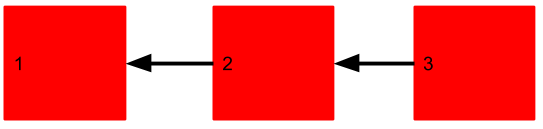
\includegraphics[scale=0.5]{figures/intermediates}
  \caption{Intermediate data sets form a linked chain.}
  \label{intermediates}
\end{figure}

\begin{figure}
  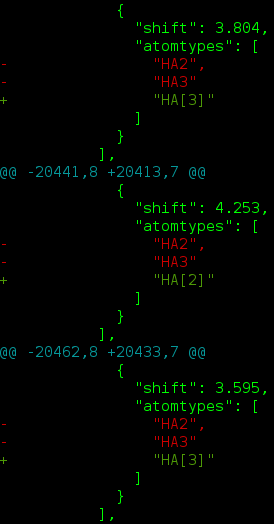
\includegraphics[scale=0.5]{figures/diff}
  \caption{Capturing intermediates allows comparison, such as diffs.}
  \label{diff}
\end{figure}

\begin{figure}
  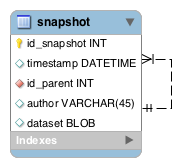
\includegraphics[scale=0.5]{figures/snapshot_model}
  \caption{A relational model of a snapshot.}
  \label{snapshot_model}
\end{figure}

\begin{figure}
  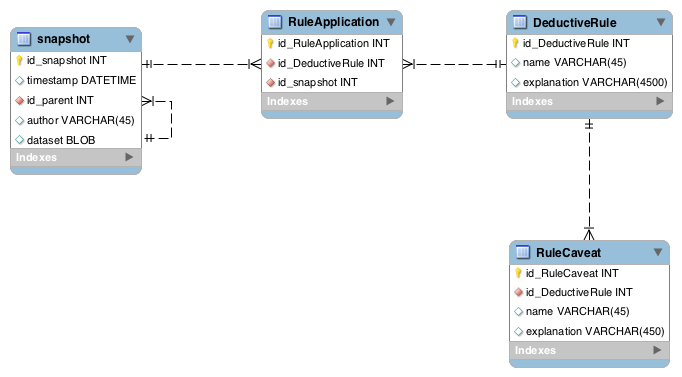
\includegraphics[scale=0.5]{figures/deduction_model}
  \caption{A relational model of a snapshot and deductions.}
  \label{deduction_model}
\end{figure}

